\documentclass[11pt,a4paper]{article}
\usepackage[utf8]{inputenc}
\usepackage[french]{babel}
\usepackage[T1]{fontenc}

\usepackage{amsmath}
\usepackage{amsfonts}
\usepackage{amssymb}

\newcommand{\NomAuteur}{Fabrice BOISSIER}
\newcommand{\TitreMatiere}{Algo et Structure de Données 1}
\newcommand{\NomUniv}{EPITA - Bachelor Cyber Sécurité}
\newcommand{\NiveauUniv}{CYBER1}
\newcommand{\NumGroupe}{CYBER1}
\newcommand{\AnneeUniv}{2022-2023}
\newcommand{\DateExam}{22 novembre 2022}
\newcommand{\TypeExam}{Examen Sujet 2}
\newcommand{\TitreExam}{\TitreMatiere}
\newcommand{\DureeExam}{2h00}
\newcommand{\MyWaterMark}{\AnneeUniv} % Watermark de protection

% Ajout de mes classes & definitions
\usepackage{MetalExam} % Appelle un .sty

% "Tableau" et pas "Table"
\addto\captionsfrench{\def\tablename{Tableau}}

%%%%%%%%%%%%%%%%%%%%%%%
%Header
%%%%%%%%%%%%%%%%%%%%%%%
\lhead{\TypeExam}							%Gauche Haut
\chead{\NomUniv}							%Centre Haut
\rhead{\NumGroupe}							%Droite Haut
\lfoot{\DateExam}							%Gauche Bas
\cfoot{\thepage{} / \pageref*{LastPage}}	%Centre Bas
\rfoot{\texttt{\TitreMatiere}}				%Droite Bas

%%%%%

\usepackage{tabularx}

\newlength{\LabelWidth}%
%\setlength{\LabelWidth}{1.3in}%
\setlength{\LabelWidth}{1cm}%
%\settowidth{\LabelWidth}{Employee E-mail:}%  Specify the widest text here.

% Optional first parameter here specifies the alignment of
% the text within the \makebox.  Default is [l] for left
% alignment. Other options are [r] and [c] for right and center
\newcommand*{\AdjustSize}[2][l]{\makebox[\LabelWidth][#1]{#2}}%


\definecolor{mGreen}{rgb}{0,0.6,0}
\definecolor{mGray}{rgb}{0.5,0.5,0.5}
\definecolor{mPurple}{rgb}{0.58,0,0.82}
\definecolor{backgroundColour}{rgb}{0.95,0.95,0.92}

\lstdefinestyle{CStyle}{
    backgroundcolor=\color{backgroundColour},
    commentstyle=\color{mGreen},
    keywordstyle=\color{magenta},
    numberstyle=\tiny\color{mGray},
    stringstyle=\color{mPurple},
    basicstyle=\footnotesize,
    breakatwhitespace=false,
    breaklines=true,
    captionpos=b,
    keepspaces=true,
    numbers=left,
    numbersep=5pt,
    showspaces=false,
    showstringspaces=false,
    showtabs=false,
    tabsize=2,
    language=C
}


\hyphenation{op-tical net-works SIGKILL}


\begin{document}

%\MakeExamTitleDuree     % Pour afficher la duree
\MakeExamTitle                   % Ne pas afficher la duree

%% \MakeStudentName    %% A reutiliser sur chaque nouvelle page

\bigskip
\bigskip

Vous devez respecter les consignes suivantes, sous peine de 0 :

\begin{itemize}
\item Lisez le sujet en entier avec attention
\item Répondez sur le sujet
\item Ne détachez pas les agrafes du sujet
\item \'Ecrivez lisiblement vos réponses (si nécessaire en majuscules)
\item Vous devez écrire dans le langage algorithmique classique ou en C (donc pas de Python ou autre)
\item Ne trichez pas
\end{itemize}

\bigskip


% Questions cours files et piles
\section{Questions (5 points)}

\subsection{(1 point) \'Ecrivez l'état des deux piles après avoir effectué ces opérations dans cet ordre (n'oubliez pas le(s) pointeur(s) de tête (et de queue) ) : }

\bigskip

%%%%%%%%%%%%%%%%% CENTRAGE
\vfill
\hspace{0pt}

\begin{center}

\begin{large}
empiler 1337, empiler 2048, dépiler, dépiler, empiler 1024, dépiler, empiler 1664
\end{large}

%\vspace{2cm}

\bigskip

\begin{figure}[ht!]
\centering
\centerline{  %%% CENTRAGE HORIZONTAL
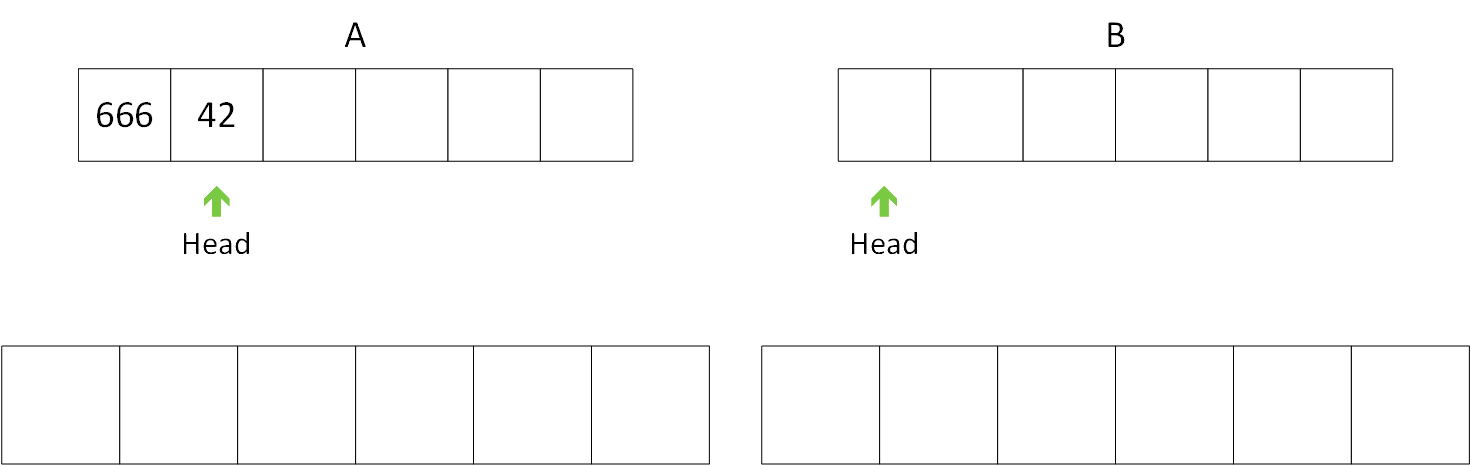
\includegraphics[scale=1]{img/Exercice1.png}
%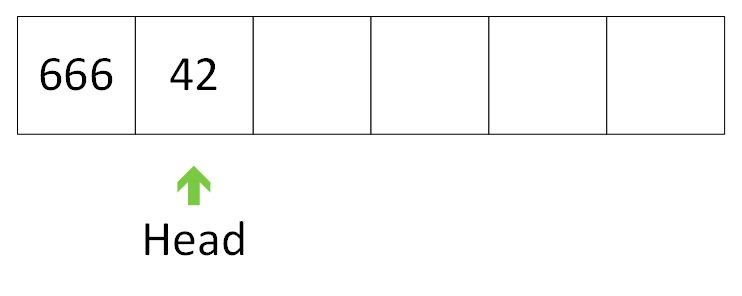
\includegraphics[scale=1,left]{img/2_elts.png}
}
%\caption{File A}
%\label{figure:1-S1-ModeleWI}
\end{figure}

\end{center}

\bigskip

%\newpage

\subsection{(0,5 point) Quel élément sortira lors du prochain \og pop \fg{} sur chaque pile ? }

\bigskip
\bigskip

%\begin{center}
\begin{Large}
A :  \hspace{8cm}  B :
\end{Large}
%\end{center}

\bigskip
\bigskip


\subsection{(0,5 point) Quel élément sortira en dernier de chaque pile ? }

\bigskip
\bigskip

%\begin{center}
\begin{Large}
A :  \hspace{8cm}  B :
\end{Large}
%\end{center}

\bigskip
\bigskip

%\vspace{5cm}

%%%%%%%%%%%%%%%%% FIN CENTRAGE

\hspace{0pt}
\vfill

\newpage

\vfillFirst

\subsection{(3 points) En admettant que l'on dispose d'une pile et que l'on insère les données \og 1 2 3 4 5 6 \fg{} dans cet ordre exclusivement, décrivez les scénarios permettant d'obtenir les sorties suivantes : }
%%% PREFERER CE TEXTE :
%\subsection{(3 points) En admettant que l'on dispose d'une pile vide et que les éléments \og 1 2 3 4 5 6 \fg{} arrivent en entrée dans cet ordre exclusivement, décrivez les scénarios permettant d'obtenir les sorties suivantes : }

\bigskip

\begin{center}
\noindent \textit{exemple : pour \og A B C \fg{} en entrée, on peut obtenir \og B C A \fg{} en sortie en faisant : \linebreak
\og push A \fg, \og push B \fg, \og pop \fg, \og push C \fg, \og pop \fg, \og pop \fg }
%%% AJOUTER CE TEXTE :
%On a bien inséré A, puis B, puis C, mais l'ordre de sortie est différent suivant les \og pop \fg}
\end{center}

\medskip


\begin{center}

\begin{large}
3, 2, 1, 4, 5, 6
\end{large}

\begin{center}
\GrilleReponseN{5}
% push 1, push 2, push 3, pop, pop, pop, push 4, pop, push 5, pop, push 6, pop
\end{center}


\begin{large}
1, 4, 3, 5, 2, 6
\end{large}

\begin{center}
\GrilleReponseN{5}
% push 1, pop, push 2, push 3, push 4, pop, pop, push 5, pop, pop, push 6, pop
\end{center}


\begin{large}
2, 4, 3, 5, 6, 1
\end{large}

\begin{center}
\GrilleReponseN{5}
% push 1, push 2, pop, push 3, push 4, pop, pop, push 5, pop, push 6, pop, pop
\end{center}

\end{center}

\vfillLast

%
\section{Algorithmes (15 points)}


\subsection{(1,5 point) \'Ecrivez une structure de données \og \textit{my\_stack\_t} \fg{} pouvant servir de pile et stockant les éléments dans un tableau }

\bigskip

\begin{center}
\GrilleReponseN{10}
\end{center}

\bigskip

\subsection{(1,5 point) \'Ecrivez une structure de données \og \textit{my\_queue\_p} \fg{} pouvant servir de file et stockant les éléments dans une liste chaînée avec pointeurs }

\bigskip

\begin{center}
\GrilleReponseN{10}
\end{center}



\newpage

\subsection{(3 points) \'Ecrivez une fonction \og \textit{push} \fg{} pouvant servir à empiler un élément dans votre précédente structure \og \textit{my\_stack\_t} \fg{} }

\bigskip

\begin{center}
%%\LigneReponseQuarante
%\LigneReponseTrente
%\LigneReponseCinq
%\LigneReponseTrois

\GrilleReponseN{24}
\end{center}

\newpage

\subsection{(3 points) \'Ecrivez une fonction \og \textit{pop} \fg{} pouvant servir à dépiler un élément dans votre précédente structure \og \textit{my\_stack\_t} \fg{} }

\bigskip

\begin{center}
\GrilleReponseN{24}
\end{center}

\bigskip



\newpage

\subsection{(3 points) \'Ecrivez une fonction \og \textit{enqueue} \fg{} pouvant servir à enfiler un élément dans votre précédente structure \og \textit{my\_queue\_p} \fg{} }

\bigskip

\begin{center}

\GrilleReponseN{24}
\end{center}

\newpage

\subsection{(3 points) \'Ecrivez une fonction \og \textit{dequeue} \fg{} pouvant servir à défiler un élément dans votre précédente structure \og \textit{my\_queue\_p} \fg{} }

\bigskip

\begin{center}
\GrilleReponseN{24}
\end{center}

\bigskip

\end{document}
